\documentclass[11pt]{article}
\pagestyle{plain}

% \pgfplotsset{compat=1.18}
\usepackage[margin=1in]{geometry}
\usepackage{amsmath,amsfonts,amssymb,amsthm}
\usepackage[ruled,vlined,linesnumbered,commentsnumbered]{algorithm2e}
\SetKwInput{KwIn}{Input}
\SetKwInput{KwOut}{Output}
\SetKwInput{KwGlobal}{Global variable}
\SetKwInput{KwOracle}{Oracle}
\SetKwComment{Comment}{// }{}
\usepackage{graphicx}
\usepackage{enumerate}
\usepackage{bbm}
\usepackage{verbatim}
\usepackage{hyperref,color}
\usepackage[capitalize,nameinlink]{cleveref}
\usepackage[dvipsnames]{xcolor}
\hypersetup{
	colorlinks=true,
	pdfpagemode=UseNone,
	citecolor=OliveGreen,
	linkcolor=NavyBlue,
	urlcolor=Magenta,
	pdfstartview=FitW
}
\usepackage{appendix}
\usepackage{makecell}
\usepackage{tablefootnote}
\crefname{appsec}{Appendix}{Appendices}
\usepackage{tikz}
\usepackage{pgfplots}
\usepackage{xifthen}
\usepackage{subcaption}
\usepackage{hhline}
\usepackage{listings}

\theoremstyle{plain}
\newtheorem{theorem}{Theorem}[section]
\newtheorem{proposition}[theorem]{Proposition}
\newtheorem{lemma}[theorem]{Lemma}
\newtheorem{corollary}[theorem]{Corollary}
\newtheorem{conjecture}[theorem]{Conjecture}
\newtheorem{problem}[theorem]{Problem}
\newtheorem{claim}[theorem]{Claim}
\newtheorem{fact}[theorem]{Fact}

\theoremstyle{definition}
\newtheorem{definition}[theorem]{Definition}
\newtheorem{example}[theorem]{Example}
\newtheorem{observation}[theorem]{Observation}
\newtheorem{assumption}[theorem]{Assumption}
\newtheorem*{assumption*}{Assumption}
\newtheorem{condition}[theorem]{Condition}

\theoremstyle{remark}
\newtheorem{remark}[theorem]{Remark}

\crefname{lemma}{Lemma}{Lemmas}
\crefname{theorem}{Theorem}{Theorems}
\crefname{definition}{Definition}{Definitions}
\crefname{fact}{Fact}{Facts}
\crefname{claim}{Claim}{Claims}
\crefname{proposition}{Proposition}{Propositions}


\newcommand{\dif}{\,\mathrm{d}}
%\newcommand{\E}{\mathbb{E}}
%\newcommand{\Var}{\mathrm{Var}}
\newcommand{\Cov}{\mathrm{Cov}}
\newcommand{\MI}{\mathrm{I}}
%\newcommand{\Ent}{\mathrm{Ent}}
\newcommand{\ind}{\mathbbm{1}}
\newcommand{\allone}{\mathbf{1}}
\newcommand{\tr}{\mathrm{tr}}
\newcommand{\wt}{\mathrm{weight}}
\DeclareMathOperator*{\argmax}{arg\,max}
\newcommand{\norm}[1]{\left\lVert #1 \right\rVert}
\newcommand{\TV}[2]{\left\|#1 - #2\right\|_{\mathrm{TV}}}
\newcommand{\ceil}[1]{\left\lceil #1 \right\rceil}
\newcommand{\floor}[1]{\left\lfloor #1 \right\rfloor}
\newcommand{\ip}[2]{\left\langle #1 , #2 \right\rangle}
\newcommand{\grad}{\nabla}
\newcommand{\hessian}{\nabla^2}
\newcommand{\trans}{\intercal}
\newcommand{\diag}{\mathrm{diag}}
\newcommand{\poly}{\mathrm{poly}}
\newcommand{\dist}{\mathrm{dist}}
\newcommand{\sgn}{\mathrm{sgn}}
\newcommand{\fpras}{\mathsf{FPRAS}}
\newcommand{\fpaus}{\mathsf{FPAUS}}
\newcommand{\fptas}{\mathsf{FPTAS}}

\newcommand{\eps}{\varepsilon}

\newcommand{\N}{\mathbb{N}}
\newcommand{\Z}{\mathbb{Z}}
\newcommand{\Q}{\mathbb{Q}}
\newcommand{\R}{\mathbb{R}}
\newcommand{\C}{\mathbb{C}}

\renewcommand{\AA}{\mathcal{A}}
\newcommand{\BB}{\mathcal{B}}
\newcommand{\CC}{\mathcal{C}}
\newcommand{\DD}{\mathcal{D}}
\newcommand{\EE}{\mathcal{E}}
\newcommand{\FF}{\mathcal{F}}
\newcommand{\GG}{\mathcal{G}}
\newcommand{\HH}{\mathcal{H}}
\newcommand{\II}{\mathcal{I}}
\newcommand{\JJ}{\mathcal{J}}
\newcommand{\KK}{\mathcal{K}}
\newcommand{\LL}{\mathcal{L}}
\newcommand{\MM}{\mathcal{M}}
\newcommand{\NN}{\mathcal{N}}
\newcommand{\OO}{\mathcal{O}}
\newcommand{\PP}{\mathcal{P}}
\newcommand{\QQ}{\mathcal{Q}}
\newcommand{\RR}{\mathcal{R}}
\renewcommand{\SS}{\mathcal{S}}
\newcommand{\TT}{\mathcal{T}}
\newcommand{\UU}{\mathcal{U}}
\newcommand{\VV}{\mathcal{V}}
\newcommand{\WW}{\mathcal{W}}
\newcommand{\XX}{\mathcal{X}}
\newcommand{\YY}{\mathcal{Y}}
\newcommand{\ZZ}{\mathcal{Z}}

\newcommand{\KL}[2]{D_{\mathrm{KL}} \left( #1 \,\Vert\, #2 \right)}
\newcommand{\KLbig}[2]{D_{\mathrm{KL}} \left( #1 \,\big\Vert\, #2 \right)}
\newcommand{\KLBig}[2]{D_{\mathrm{KL}} \left( #1 \,\Big\Vert\, #2 \right)}

\newcommand{\SKL}[2]{D_{\mathrm{SKL}} \left( #1 \,\Vert\, #2 \right)}
\newcommand{\SKLbig}[2]{D_{\mathrm{SKL}} \left( #1 \,\big\Vert\, #2 \right)}
\newcommand{\SKLBig}[2]{D_{\mathrm{SKL}} \left( #1 \,\Big\Vert\, #2 \right)}

\newcommand{\qandq}{\quad\text{and}\quad}
\newcommand{\supp}{\mathrm{supp}}

\newcommand{\DKL}[2]{\-D_{\-{KL}}\left(#1 \parallel #2\right)}
\newcommand{\DTV}[2]{\-D_{\mathrm{TV}}\left({#1},{#2}\right)}
% \newcommand{\dist}{\mathrm{dist}}
\newcommand{\e}{\mathrm{e}}
\renewcommand{\epsilon}{\varepsilon}
\renewcommand{\emptyset}{\varnothing}
% \newcommand{\norm}[1]{\left\Vert#1\right\Vert}
\newcommand{\set}[1]{\left\{#1\right\}}
\newcommand{\tuple}[1]{\left(#1\right)} 
% \newcommand{\eps}{\varepsilon}
\newcommand{\inner}[2]{\left\langle #1,#2\right\rangle}
\newcommand{\tp}{\tuple}
\newcommand{\ol}{\overline}
\newcommand{\abs}[1]{\left\vert#1\right\vert}
\newcommand{\ctp}[1]{\left\lceil#1\right\rceil}
\newcommand{\ftp}[1]{\left\lfloor#1\right\rfloor}
\newcommand{\Ind}[1]{\-{Ind}_{#1}}
\newcommand{\todo}[1]{{\color{red} TODO: #1}}

\newcommand{\Cor}{\Psi^{\mathrm{sym}}}
\newcommand{\cor}{\Psi^{\-{cor}}}
\newcommand{\Inf}{\Psi}
% \newcommand{\diag}{\-{diag}}

\def\*#1{\boldsymbol{#1}} % Use \*A for \mathbf{A}
\def\+#1{\mathcal{#1}} % Use \+A for \mathcal{A}
\def\-#1{\mathrm{#1}} % Use \-A for \mathrm{A}
\def\=#1{\mathbb{#1}} % Use \^A for \mathbb{A}
\def\!#1{\mathfrak{#1}} % Use \!A for \mathfrak{A}

\newcommand*\diff{\mathop{}\!\mathrm{d}}

% probability
% \DeclareMathOperator*{\oPr}{\mathbf{Pr}}
\def\oPr{\mathop{\mathrm{Pr}}}
\renewcommand{\Pr}[2][]{ \ifthenelse{\isempty{#1}}
  {\oPr\left[#2\right]}
  {\oPr_{#1}\left[#2\right]} } % Use \Pr[a]{b} for \mathbf{Pr}_a[b], \Pr{b} for  \mathbf{Pr}[b]

% expectation: relies on the package "dsfont"
% \DeclareMathOperator*{\oE}{\mathbb{E}}
\def\oE{\mathop{\mathbb{E}}}
\newcommand{\E}[2][]{ \ifthenelse{\isempty{#1}}
  {\oE\left[#2\right]}
  {\oE_{#1}\left[#2\right]} }

% variance
%\DeclareMathOperator*{\oVar}{\mathbf{Var}}
\def\oVar{\mathrm{Var}}
\newcommand{\Var}[2][]{ \ifthenelse{\isempty{#1}}
  {\oVar\left[#2\right]}
  {\oVar_{#1}\left[#2\right]} }

% entropy
% \DeclareMathOperator*{\oEnt}{\mathbf{Ent}}
\def\oEnt{\mathrm{Ent}}
\newcommand{\Ent}[2][]{ \ifthenelse{\isempty{#1}}
  {\oEnt\left[#2\right]}
  {\oEnt_{#1}\left[#2\right]} }

\newcommand{\PhiEnt}[2][]{ \ifthenelse{\isempty{#1}}
  {\oEnt^\phi\left[#2\right]}
  {\oEnt^\phi_{#1}\left[#2\right]} }


\newenvironment{Exampleparagraph}[1][]
{
    \par 
    \noindent 
    \textbf{\color{blue} #1}
    \par 
    \vspace{0.5em} 
    \itshape 
}
{
    \par 
    \vspace{1em} 
}

%\input{local-macro}

\newcommand{\RED}[1]{\textcolor{red}{#1}}

\newcommand{\bern}[1]{\mathrm{Bern}\left(#1\right)}
\newcommand{\pll}{\parallel}



\title{CS 7545 F26, Computational Mini Project 2}
\date{Due on September 24, 2026}
\author{{\textbf{Zejia Chen}} \\ \textbf{GTID: 904178159}}

\pgfplotsset{compat=1.18} 
\begin{document}

\maketitle

\section*{Part 1}
The following figures are visualization of the distribution and dataset.
\begin{figure}[htbp]
    \centering
    \begin{subfigure}{0.49\textwidth}
        \centering
        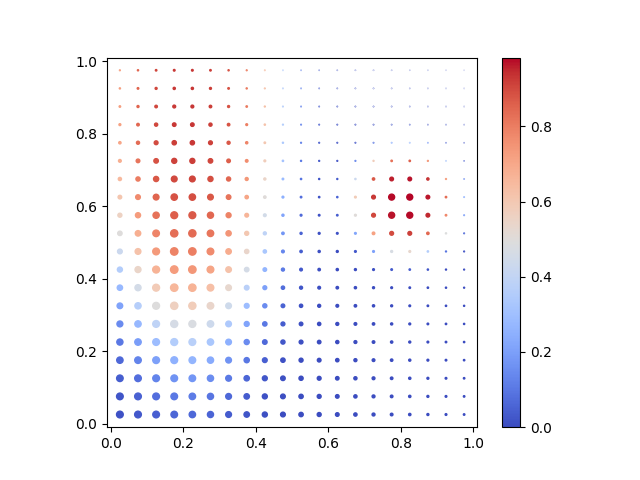
\includegraphics[
            width=\textwidth,
            trim={1.9cm 0 2cm 0},
            clip
        ]{part1/part1_distribution.png}
    \end{subfigure}
    \hfill
    \begin{subfigure}{0.49\textwidth}
        \centering
        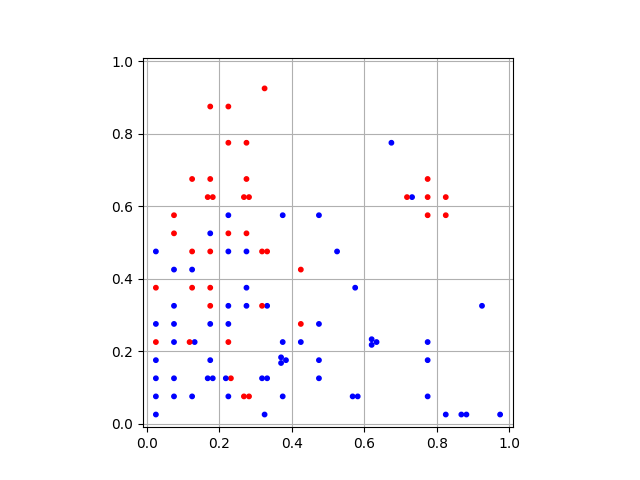
\includegraphics[
            width=\textwidth,
            trim={1.9cm 0 2cm 0},
            clip
        ]{part1/part1_dataset.png}
    \end{subfigure}
    \caption{Visualization of the distribution $D$ and the dataset $S$.}
\end{figure}
\newpage
\section*{Part 2}
\subsection*{Part 2.a}
The following figures are visualization of the distribution and dataset with \textbf{seed 4}.
\begin{figure}[htbp]
    \centering
    \begin{subfigure}{0.49\textwidth}
        \centering
        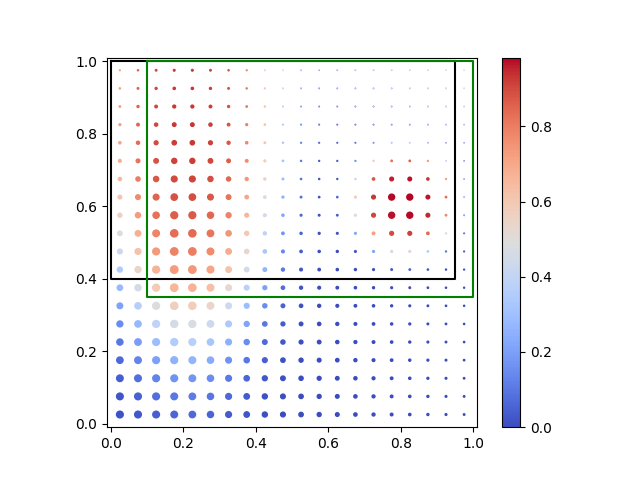
\includegraphics[
            width=\textwidth,
            trim={1.9cm 0 2cm 0},
            clip
        ]{part2/part2a/part2a_distribution4.png}
    \end{subfigure}
    \hfill
    \begin{subfigure}{0.49\textwidth}
        \centering
        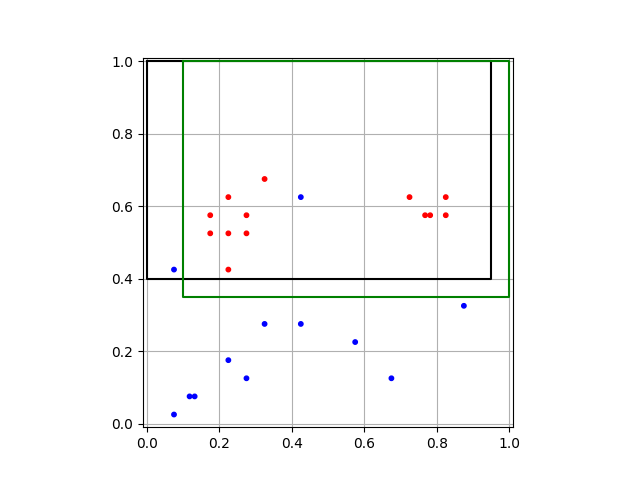
\includegraphics[
            width=\textwidth,
            trim={1.9cm 0 2cm 0},
            clip
        ]{part2/part2a/part2a_dataset4.png}
    \end{subfigure}
    \caption{Visualization of the distribution $D$ and the dataset $S$ with \textbf{seed 4}.}
\end{figure}
\\And the loss values with different seeds are as follows. 
\begin{figure}[htbp!]
    \centering
    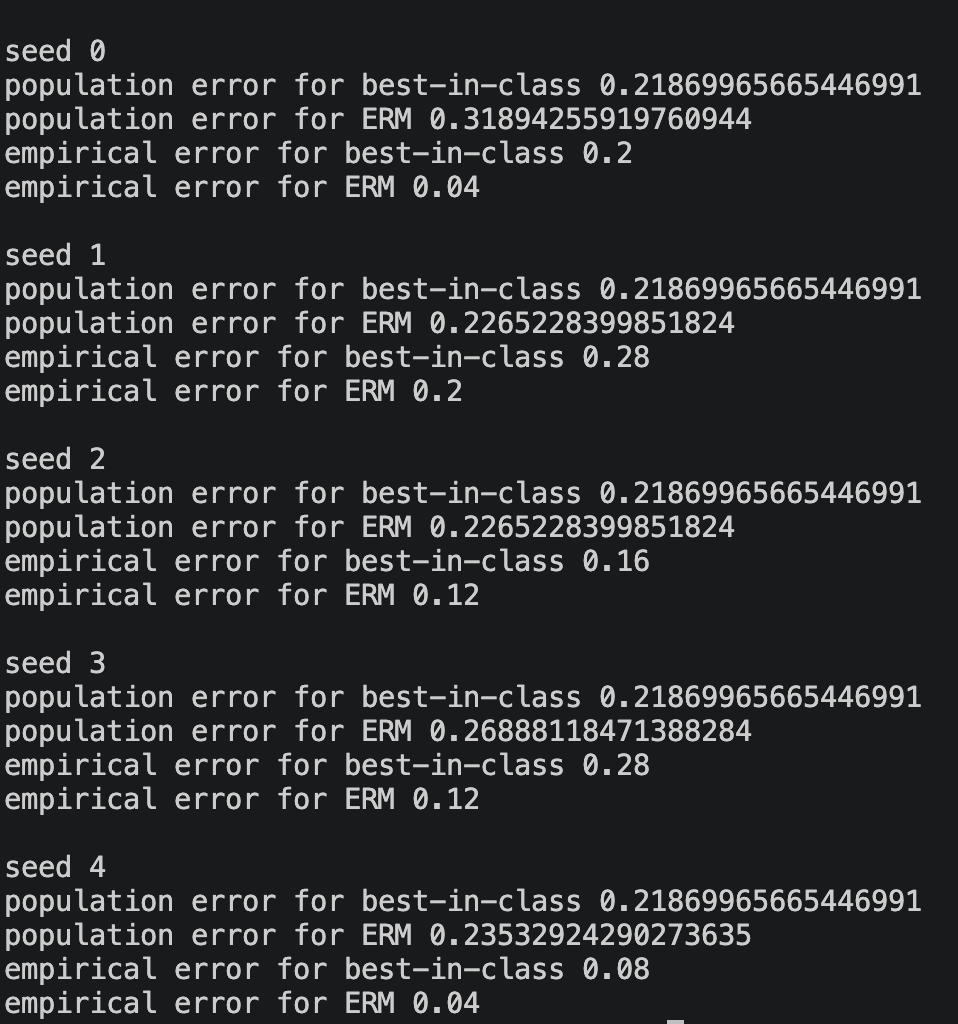
\includegraphics[width=.45\textwidth]{part2/part2a/error.png}
    \caption{The loss values with different seeds.}
\end{figure}
\begin{itemize}
    \item [1.] The empirical risk minimizer $\hat h_S$ changes with the sample. For example, the rectangle selected with seed $0$ covers a small region on the left, which is quite different from the rectangles selected with seeds $1$ and $2$.
    By the definition of the error, the ERM covers most red points (positive points) and excludes most blue points (negative points) and therefore, ERM is highly depend on the samples and changes with samples.
    
    \item [2.] 
    The loss values satisfy $L(h^\star)\leq L(\hat h_S)$ and $\hat L_S(\hat h_S)\leq\hat L_S(h^\star)$ for every seed, which follows from the minimality.
    No fixed ordering is guaranteed between a hypothesis’s empirical and population losses.
    
    In most seeds, the empirical error for ERM is relatively close to the empirical error for best-in-class and the population error for ERM approaches the population error of the best-in-class as well.
    That is because the behavior of dataset is close to the underlying distribution by concentration.
    But with only 25 samples, noticeable gaps can remain. 

    For seed $0$, the empirical error of ERM is much less than that of best-in-class but the population error of ERM is large.
    The underlying reason is that the empirical minimizer may overfit in the dataset $S$.
\end{itemize}

\subsection*{Part 2.b}
The following figures are visualization of the distribution and dataset with \textbf{seed 4}.
\begin{figure}[htbp]
    \centering
    \begin{subfigure}{0.49\textwidth}
        \centering
        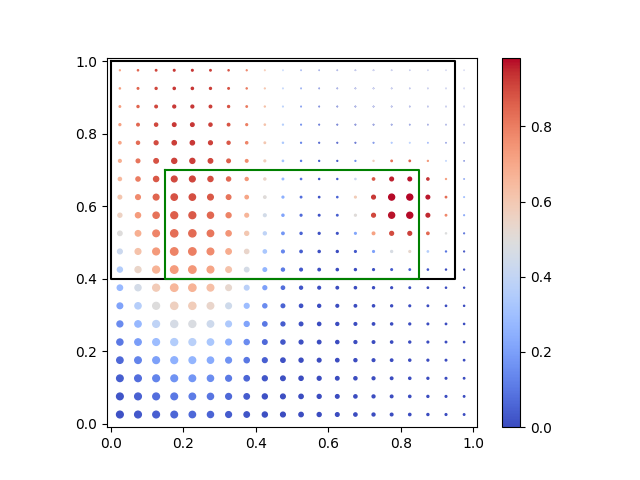
\includegraphics[
            width=\textwidth,
            trim={1.9cm 0 2cm 0},
            clip
        ]{part2/part2b/part2b_distribution4.png}
    \end{subfigure}
    \hfill
    \begin{subfigure}{0.49\textwidth}
        \centering
        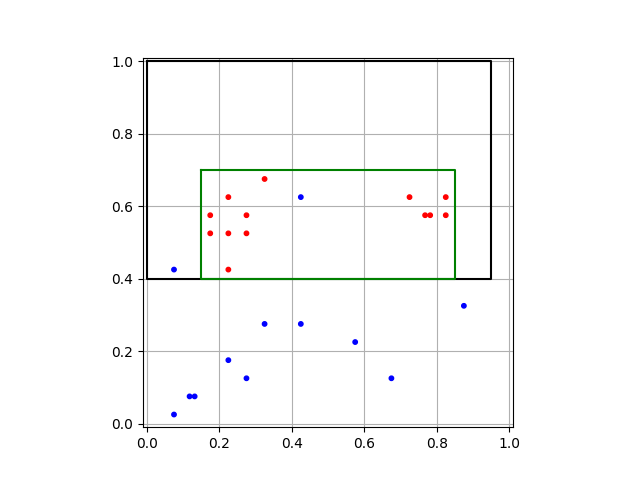
\includegraphics[
            width=\textwidth,
            trim={1.9cm 0 2cm 0},
            clip
        ]{part2/part2b/part2b_dataset4.png}
    \end{subfigure}
    \caption{Visualization of the distribution $D$ and the dataset $S$ with \textbf{seed 4}.}
\end{figure}
\\And the loss values with different seeds are as follows. 
\begin{figure}[htbp!]
    \centering
    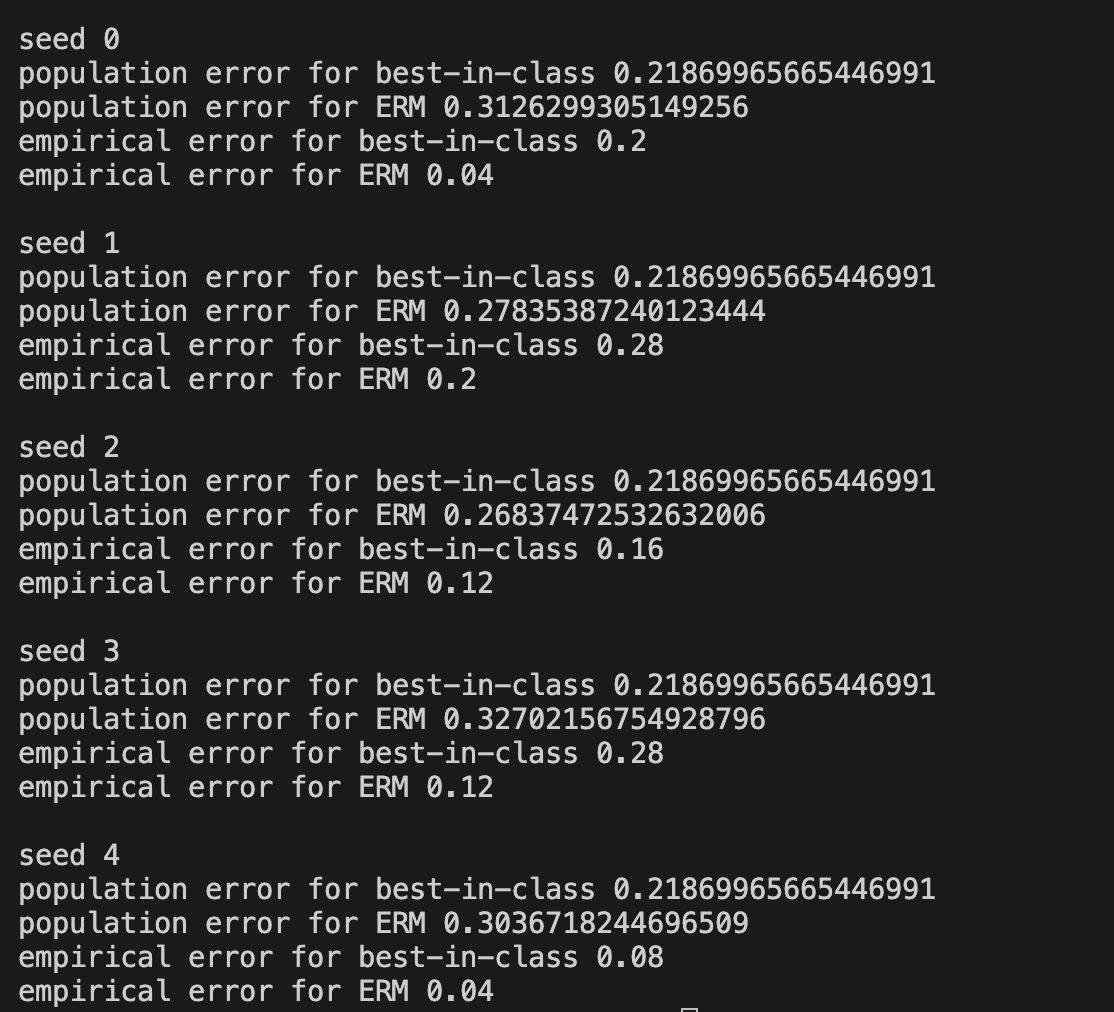
\includegraphics[width=.45\textwidth]{part2/part2b/error.png}
    \caption{The loss values with different seeds.}
\end{figure}

\newpage
\begin{itemize}
    \item [1.] It changes the choice among hypotheses with the same minimum empirical loss. 
    The minimum empirical loss is unchanged for each seed, but the selected minimizer rectangle may change.
    For most seeds, the new rectangles here are a subset of the Part 2.a rectangle; seed 2 is an exception.

    Due to the different tie-breaking choice, the population loss is also changed in either direction.
    In these experiments, population loss decreases slightly for seed $0$ and increases for seeds $1,2,3,4$.
    Hence, choosing a smaller empirical minimizer does not necessarily reduce population loss.
\end{itemize}

\section*{Part 3}
\subsection*{Part 3.a}
\begin{figure}[htbp!]
    \centering
    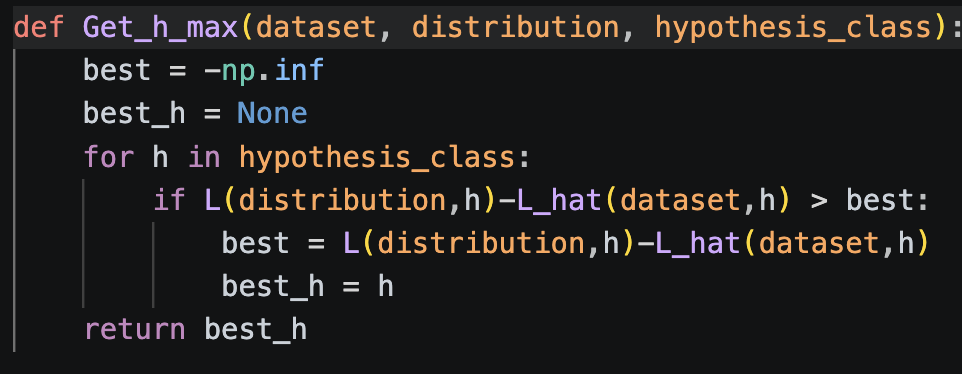
\includegraphics[width=.9\textwidth]{part3/code.png}
    \caption{Codes of \texttt{Get\_h\_max(dataset, distribution, hypothesis\_class)}}
\end{figure}
\subsection*{Part 3.b}
The following figure is the histogram with \textbf{seed 1}.
\begin{figure}[htbp!]
    \centering
    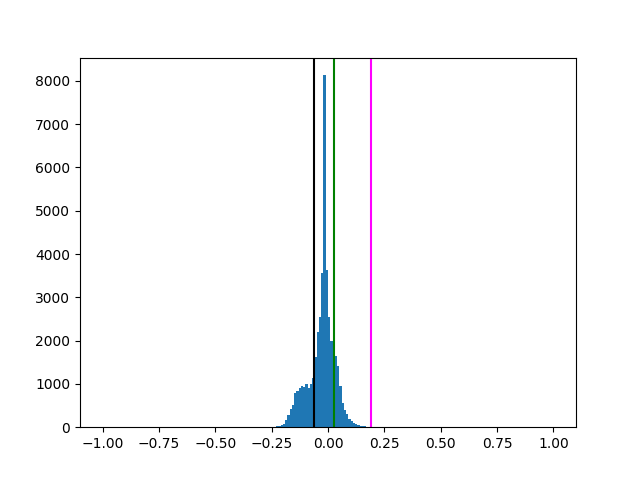
\includegraphics[width=.68\textwidth]{part3/part3_histogram1.png}
    \caption{Histogram of $L(h) - \hat L_S(h)$ with \textbf{seed 1}, the black line is $h^\star$ and the green line is $\hat h_S$.}
\end{figure}

\begin{itemize}
    \item [1.] The histogram has a concentrated peak with tails that decrease in both directions and can be asymmetric. It is centered near zero ($\pm 0.25$).
    \item [2.] The peak and tails shift as the sample changes.
    For example, the peak is near $0.25$ for seed $0$ and near $-0.1$ for seed $4$.
    That is because many hypotheses make similar predictions, so one sample can shift many of their gaps in the same direction.
    \item [3.] Since $h^\star$ is fixed before sampling, we have that $\E{L(h^\star) - \hat L_S(h^\star)} = 0$, where the expectation is over $S$.
    Like other hypotheses fixed before sampling, $h^\star$ has no consistent position relative to the histogram peak: its gap may be near or far from the peak, depending on the sample.
    \item [4.] $\hat h_S$ is chosen based on samples $S$ and its empirical loss is optimistically low.
    The gap $L(\hat h_S) - \hat L_S(\hat h_S)$ therefore tends to be positive and toward the right side of the histogram.
\end{itemize}
\newpage
\section*{Part 4}
For $n = 25$, RHS is equal to $0.52325801159636$.
For $n = 100$, RHS is equal to $0.261629005798181$.
The values of the LHS for the first $5$ seeds with $n=25,100$ are as follows,
\begin{figure}[htbp!]
    \centering
    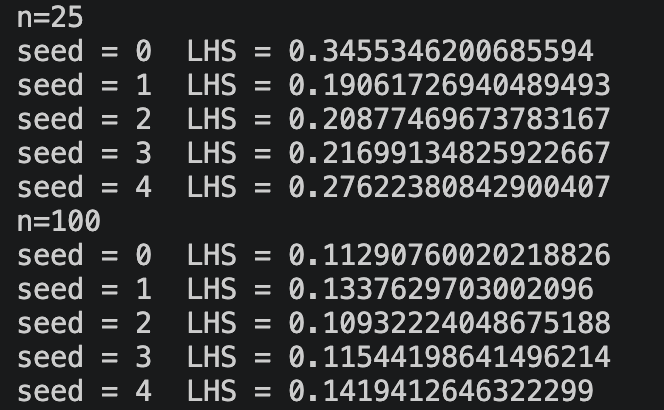
\includegraphics[width=.68\textwidth]{part4/LHS.png}
    \caption{The values of the LHS for the first 5 seeds with $n=25,100$.}
\end{figure}
\begin{itemize}
    \item [1.] The bound is greater than all measured corresponding empirical values, which matches our expectation.
    That is, with probability at least $0.95$ over a randomly drawn sample, the bound is the upper bound of the empirical value.
    On average, the empirical values are roughly half of the corresponding bound, so the bounds are valid for these samples but not particularly tight.
    \item [2.] 
    The bound is proportional to $1/\sqrt n$, so increasing $n$ from $25$ to $100$ halves it exactly.
    The average empirical value also falls by about half, from $0.2476$ to $0.12267$.

    The observed empirical value is smaller on average at \(n=100\), consistent with stronger concentration, which matches our expectation: the empirical value has a negative correlation with $n$.
    Therefore, as the $n$ increase, the gap between our bound and the empirical value will decrease.
\end{itemize}
\end{document} 